\section{Description of a use case model}
\textbf{System:} Calculator System \\ \\
\textbf{Actor:} Calculator User \\ \\
\textbf{User cases: }
\begin{enumerate}
  \item Evaluate Expression
  \item Evaluate Irrational Number Value
  \item Evaluate Irrational Algebraic Expression
  \item Evaluate Irrational Arithmetic Expression
  \item Evaluate Area of Regular Octagon Expression
  \item Evaluate Area of Circle Expression
  \item Save Value of Evaluated Expression
  \item Display Answer \\
\end{enumerate}
\textbf{Relationships between use cases:}
\begin{enumerate}
  \item Evaluate Irrational Number Value, Evaluate Irrational Algebraic Expression, Evaluate Irrational Arithmetic Expression, Evaluate Area of Regular Octagon Expression, Evaluate Area of Circle Expression \textbf{are-kind of} Evaluate Expression \textbf{(Generalization Relationship)}.
  \item Save Value of Evaluated Expression \textbf{extends} Evaluate Irrational Number Value, Evaluate Irrational Algebraic Expression, Evaluate Irrational Arithmetic Expression, Evaluate Area of Regular Octagon Expression, Evaluate Area of Circle Expression \textbf{based on the condition} if user choose to save value of evaluated expression.
  \item Evaluate Expression \textbf{includes} Display Answer. \\
\end{enumerate}
\textbf{Relationships between actor and use cases:}
Calculator user Evaluates Expression.

\section{View 1: Use case model diagram}
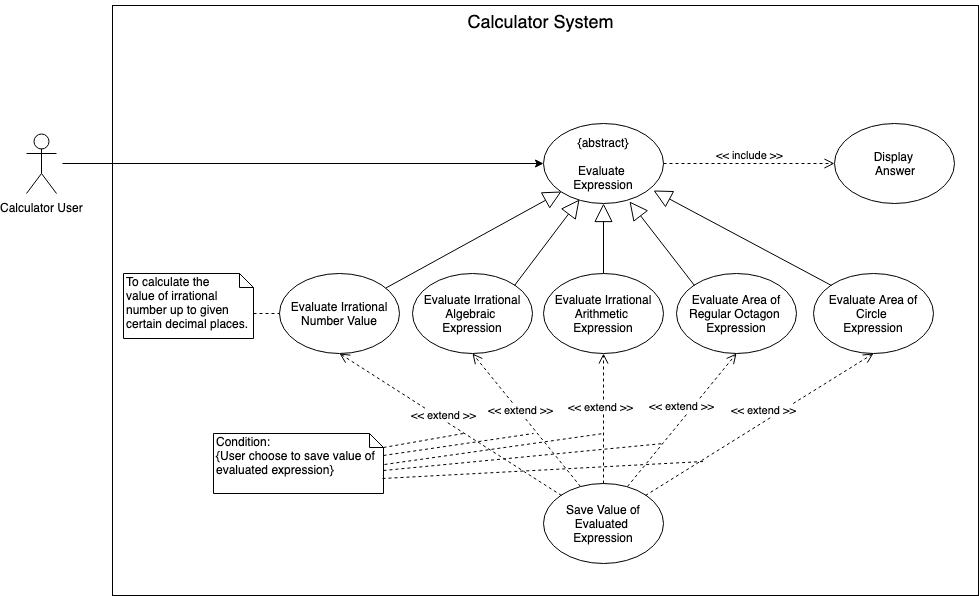
\includegraphics[width=1.0\textwidth]{images/usecasemodel.png}

\section{View 2: Activity Diagram}
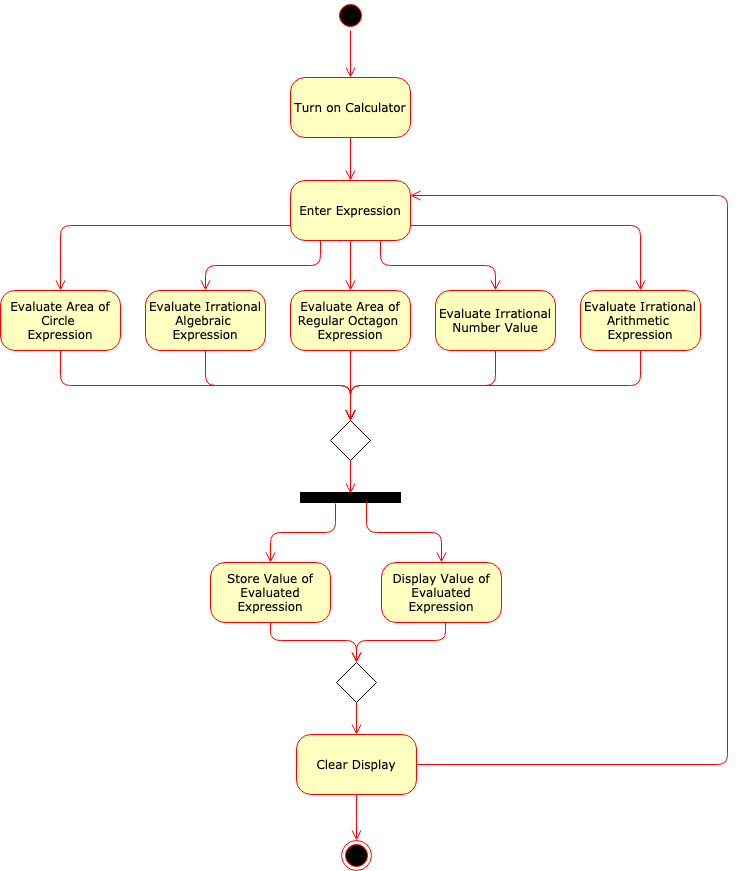
\includegraphics[width=1.0\textwidth]{images/activitydiagram.png}

\section{Scenarios of use cases}
\textbf{Scenario 1:} Following UML Sequence Diagram shows a scenario that is the evaluation of any general expression.\\ \\
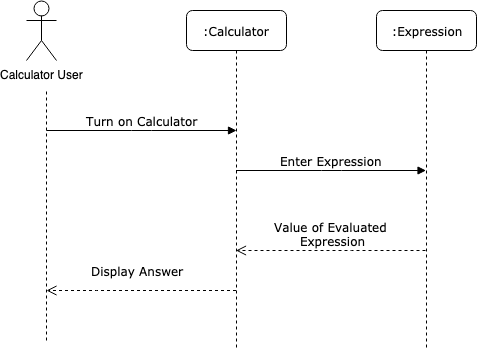
\includegraphics[width=1.0\textwidth]{images/s1.png} \\ \\
\textbf{Scenario 2:} Following UML Sequence Diagram shows a scenario that is the evaluation of the expression to find the area of regular octagon using the Silver Ratio number.\\ \\
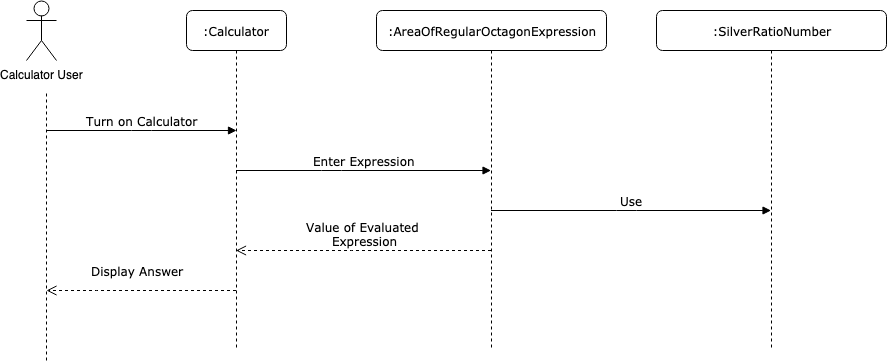
\includegraphics[width=1.0\textwidth]{images/s2.png} \\ \\
\textbf{Scenario 3:} Following UML Sequence Diagram shows a scenario that is the evaluation of the expression to find the area of circle using the Pi number.\\ \\
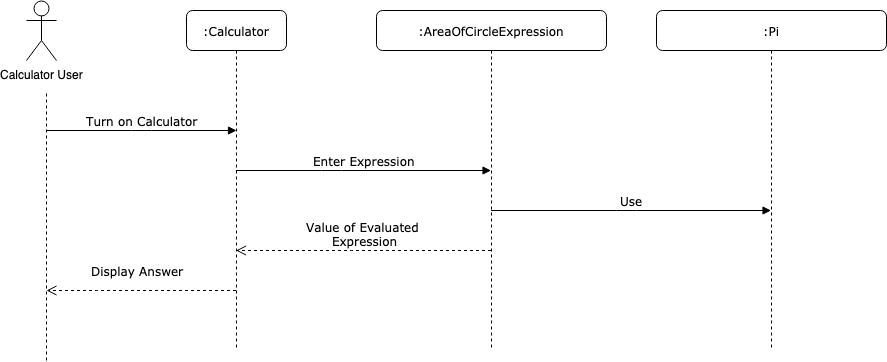
\includegraphics[width=1.0\textwidth]{images/s3.png}

